\chapter{Trabalhos relacionados}\label{cap_trabalhos_relacionados}

Neste capítulo serão discutidos os trabalhos relacionados à compressão de CNN com foco em dispositivos
embarcados.

\section{Trabalhos acadêmicos}

Os seguintes critérios de busca foram utilizados para filtrar os trabalhos acadêmicos:

\begin{itemize}
	% TODO: Olhar
	\item Portal de periódicos utilizada foi a CAPES CAFE.
	\item A string de busca foi a seguinte: "face recognition" and "esp32".
	\item O seguintes filtros foram utilizados:
	\begin{itemize}
		\item Idioma: Inglês.
		\item Revisado por pares: Sim.
	\end{itemize}
---
	\item Os artigos devem ser relacionado ao tema de CNN com compressão para sistemas embarcados.
	\item Trabalhos publicados entre 2020 e 2023.
	\item Trabalhos escritos em inglês.

	As bases utilizadas foram: IEE Eletronic Library, ACM Digital Library e Science Citation Index Expanded.
	Utilizando a seguinte string de busca:
	\item "CNN"  AND "EMBEDDED" AND "Edge devices" AND ("Pruning" OR "Knowledge distillation" OR "Quantization")
\end{itemize}

\subsection{\textit{A Resource Constrained Pipeline Approach to Embed Convolutional Neural Models (CNN)}}
O objetivo deste trabalho de dissertação \cite{rafael} é elaborar um modelo de detecção de placas de trânsito que seja
computacionalmente e energeticamente barato. Para atingir esse objetivo, foi elaborada uma pipeline de compressão,
começando pela destilação de conhecimento, e partindo para poda e quantização.

O resultado alcançado foi uma CNN capaz de detectar placas de trânsito, consumindo 59KB de espaço, com $85,91\%$ de
acurácia e F1-Score igual a $85,80\%$, atingindo um tempo de inferência de 80 ms no ESP32 e 83 ms no ESP32-2.

\subsection{\textit{IMPROVED FACE DETECTION ACCURACY USING HAAR CASCADE CLASSIFIER METHOD AND ESP32-CAM FOR IOT-BASED HOME DOOR SECURITY}}

\subsection{\textit{Intelligent security system based on face recognition and IoT}}
Este artigo \cite{bagchi20222133} tem como objetivo desenvolver um protótipo de sistema de segurança baseado em reconhecimento facial,
utilizando \textit{Internet of Things} (IOT). Para atingir esse objetivo, os autores utilizam um ESP32-CAM como componente
principal para realizar a coleta e reconhecimento da face.

% TODO:Melhorar
O resultado alcançado foi um protótipo que é capaz de verificar se a face capturada é conhecida, caso seja, ela acende um
LED verde, caso contrário um LED vermelho é ligado. Além disso, foi levantada uma lista de pontos fortes, fracos, ameaças
e oportunidade do protótipo.

\begin{center}
\begin{table}[htb]
\centering
\ABNTEXfontereduzida
\caption[Pontos fortes, fracos, oportunidades e ameaças]{Pontos fortes, fracos, oportunidades e ameaças}
\label{tabela_swot}
\begin{tabular}{ |c|c| }
	\hline
	Ponto forte & Eficiência energética \\
		    & Custo x benefício \\
		    & Design robusto \\
		    & Pode armazenar até 200 faces \\
	\hline
	Ponto fraco & Precisa de conexão com WiFi constante \\
	 	    & Alcance de detecção facial limitado \\
	\hline
	Oportunidade & Sistema de segurança com baixo custo\\
		 & Usado em sistema de atendimento \\
		 & Usado em sistema de pagamento \\
	\hline
	Ameaça & Não aplicável para usos ao ar livre \\
	\hline
\end{tabular}
\legend{Fonte: \citeonline{bagchi20222133}}
\end{table}
\end{center}

\subsection{\textit{A face recognition application for Alzheimer’s patients using ESP32‑CAM and Raspberry Pi}}
Este trabalho \cite{espcamAlzheimer} tem como objetivo, desenvolver um aparelho para auxiliar pessoas com Alzheimer,
utilizando reconhecimento facial. Para atingir esse objetivo, foi utilizada uma ESPCAM, para fazer a detecção facial
e um Raspberry Pi, para fazer o reconhecimento facial. De forma que, a câmera detecta a face, realiza um recorte
(\textit{crop}) e a envia para o servidor realizar a detecção, onde, caso seja uma face conhecida, o nome da pessoa será
falado por um alto-falante (\textit{speaker}), como é possível notar a .

\begin{figure}[htb]
	\caption {\label{pipeline_espcam}Pipeline do reconhecimento facial}
	\begin{center}
		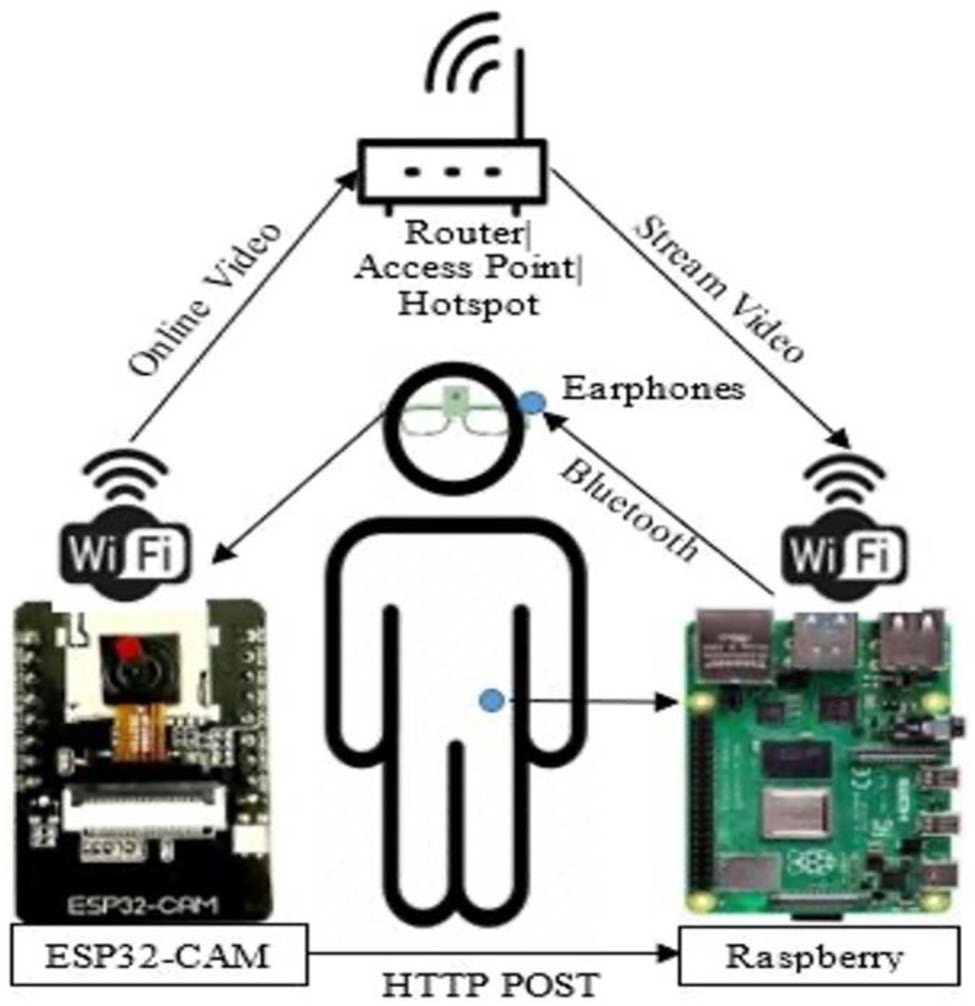
\includegraphics[scale=0.15]{Imagens/pipiline-espcam-alzheimer}
	\end{center}
	\legend {Fonte: \citeonline{bagchi20222133}}
\end{figure}
